\section{Ground-Truth Water Quality Index}
\label{sec:wqi}

\subsection{Formula}

We use the CPCB weighted-arithmetic index (\texttt{scripts/compute\_wqi.py}). For each parameter $i$ a sub-index $q_i\ge 0$ is computed, where $q_i=0$ is ideal and $q_i=100$ means exactly at the standard:
\begin{align}
  q_i &= 100\,\frac{x_i}{S_i} && \text{BOD, coliforms, turbidity, nitrate-N, EC (more is worse)} \\
  q_{\mathrm{DO}} &= 100\,\frac{14.6 - x_{\mathrm{DO}}}{14.6 - 5} && \text{DO (less is worse; 14.6 mg/L = saturation at 0\,\si{\celsius})} \\
  q_{\mathrm{pH}} &= \begin{cases} 100\,(x_{\mathrm{pH}}-7)/(8.5-7) & x_{\mathrm{pH}}\ge 7 \\ 100\,(7-x_{\mathrm{pH}})/(7-6.5) & x_{\mathrm{pH}}<7 \end{cases} && \text{pH (asymmetric CPCB band)}
\end{align}
Unit weights are $W_i = K/S_i$ with $K = 1/\sum_j (1/S_j)$, so that $\sum_i W_i = 1$. For pH the band width $8.5-6.5=2$ serves as $S_i$. The index is
\begin{equation}
  \wqi = \frac{\sum_i W_i\, \min(q_i, 100)}{\sum_i W_i}.
  \label{eq:wqi}
\end{equation}

\begin{table}[h]
\centering\small
\caption{Standard values and resulting unit weights. The four CPCB primary bathing-water criteria carry high confidence; the other four are commonly used secondary thresholds.}
\label{tab:standards}
\begin{tabular}{llrlr}
\toprule
Parameter & Standard $S_i$ & Ideal & Source & Weight $W_i$ \\
\midrule
pH & 6.5--8.5 (band 2.0) & 7.0 & CPCB bathing criteria & 0.4049 \\
BOD & 3 mg/L & 0 & CPCB bathing criteria & 0.2699 \\
DO & 5 mg/L & 14.6 & CPCB bathing criteria & 0.1620 \\
Turbidity & 10 NTU & 0 & river-WQI literature & 0.0810 \\
Nitrate-N & 10.16 mg N/L & 0 & BIS 45 mg/L NO$_3^-$, converted & 0.0797 \\
Fecal coliform & 500 MPN/100mL & 0 & CPCB bathing criteria & 0.0016 \\
EC & 1000 \si{\micro S/cm} & 0 & river-WQI literature (weakest) & 0.0008 \\
Total coliform & 5000 MPN/100mL & 0 & river-WQI literature & 0.0002 \\
\bottomrule
\end{tabular}
\end{table}

\subsection{Why the sub-indices are capped}

With the textbook uncapped formula the index is dominated by a few genuine extremes. Turbidity of 3,640 NTU at the Mahi during a monsoon flood gives $q_{\text{Turb}}=36{,}400$ and an index of 3,007. BOD of 294 mg/L on the Ganga near Munger gives an index of 2,716. The uncapped index has mean 108, median 65 and standard deviation 175 (\cref{fig:wqidist}). Capping each $q_i$ at 100, i.e.\ treating ``beyond the standard'' as ``violation'' without further extrapolation, is standard practice. It gives a well-behaved target with mean 56.1, standard deviation 14.1 and range 13.7--92.6. Because the capped index is a weighted mean of values in $[0,100]$, it cannot exceed 100, so the ``Unsuitable'' class ($>100$) is structurally empty. The uncapped variant is analysed separately in \cref{sec:res-sens}.

\begin{figure}[t]
  \centering
  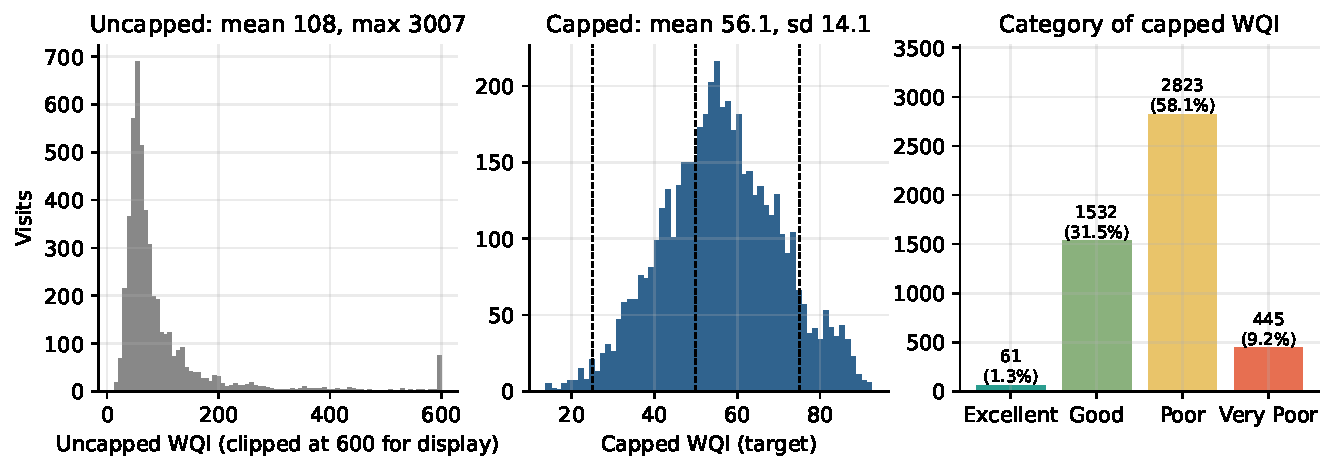
\includegraphics[width=\textwidth]{fig_eda_wqi_distribution.pdf}
  \caption{Left: uncapped index (clipped at 600 for display). Middle: capped index, the regression target, with category boundaries. Right: category distribution of the target. ``Poor'' (51--75) is the majority class at 58.1\%.}
  \label{fig:wqidist}
\end{figure}

The target categories are Excellent ($\le$25): 61 visits (1.3\%), Good (26--50): 1,532 (31.5\%), Poor (51--75): 2,823 (58.1\%) and Very Poor (76--100): 445 (9.2\%). A classifier that always predicts ``Poor'' would therefore score 58.1\% category accuracy. This is the baseline that category accuracies in \cref{sec:results} should be read against.

\subsection{What actually drives the index}
\label{sec:wqi-weights}

Because \cref{eq:wqi} is linear in the capped sub-indices, its variance decomposes \emph{exactly}:
\begin{equation}
  \operatorname{Var}(\wqi) = \sum_i \operatorname{Cov}\!\left(W_i \tilde q_i,\; \wqi\right), \qquad \tilde q_i=\min(q_i,100),
\end{equation}
so $\operatorname{Cov}(W_i\tilde q_i,\wqi)/\operatorname{Var}(\wqi)$ is the share of index variance attributable to parameter $i$, and the shares sum to one. \Cref{fig:weights} shows the three ingredients: the unit weight, the spread of the capped sub-index, and the resulting variance share.

\begin{figure}[t]
  \centering
  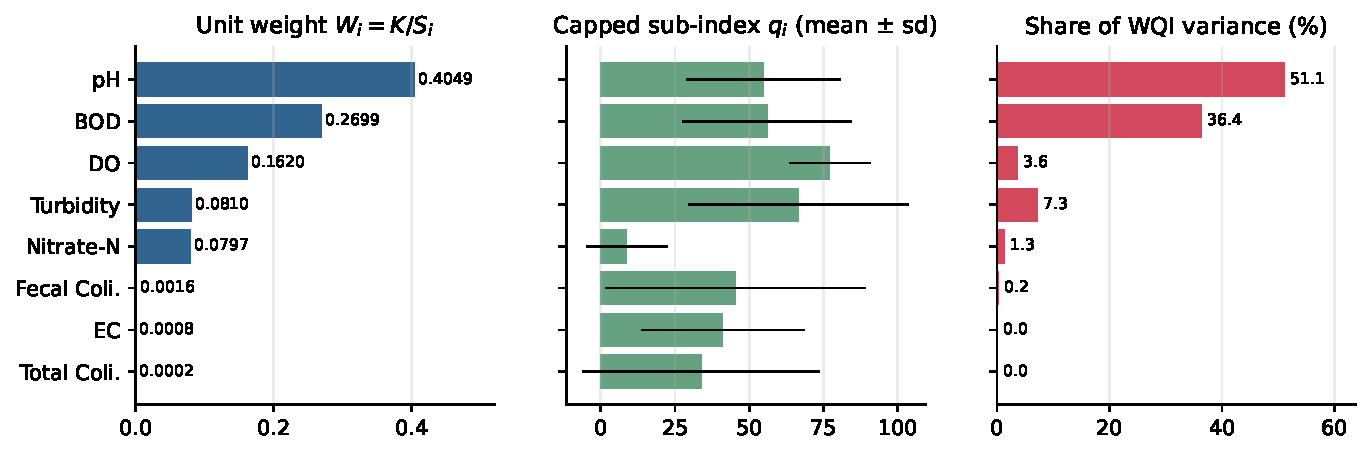
\includegraphics[width=\textwidth]{fig_eda_weights.pdf}
  \caption{Left: unit weights $W_i=K/S_i$. Middle: mean $\pm$ s.d.\ of the capped sub-indices. Right: exact share of target variance per parameter. pH and BOD account for 87.5\% of the variance; fecal coliform, EC and total coliform together for 0.24\%.}
  \label{fig:weights}
\end{figure}

\begin{keybox}[Finding 1: the CPCB weights make three of the eight parameters almost irrelevant]
pH explains 51.1\% of the index variance, BOD 36.4\%, turbidity 7.3\%, DO 3.6\% and nitrate-N 1.3\%. Fecal coliform (0.19\%), EC (0.04\%) and total coliform (0.02\%) are almost irrelevant. The reason is arithmetic, not hydrological. A weight of $1/S_i$ rewards parameters whose standard is a \emph{small number in its unit}: 2 pH units or 3 mg/L, versus 500 or 5,000 MPN/100\,mL. Fecal coliform exceeds its standard on a third of visits and still cannot move the index.
\end{keybox}

This has two consequences that shape the rest of the report. First, it predicts that adding fecal coliform and EC to \sub{S3} (to form the originally proposed \sub{S5}) will barely improve accuracy, and that turbidity and nitrate-N are the parameters worth adding. Second, it means the CPCB-weighted index is effectively blind to bacterial contamination. A reduced-parameter model that reproduces the index faithfully inherits that blindness. We return to this public-health caveat in \cref{sec:discussion}, and test the alternative of equal weights in \cref{sec:res-sens}.

Two further conventions inflate the index for ordinary river water. A typical river pH of 7.8 scores $q_{\mathrm{pH}}=53$ because the ideal is 7.0. A healthy DO of 7.2 mg/L scores $q_{\mathrm{DO}}=77$ because the ideal is 14.6 mg/L, the saturation value at 0\,\si{\celsius}. These conventions are why 67\% of visits fall in Poor or Very Poor even though only 12\% exceed the BOD standard. The categories are therefore best read as relative positions on this particular scale, not as absolute verdicts.
